\begin{frame}
  \frametitle{Future Work}
  We have shown that PyRe allows Cyclus to simulate a simple pyroprocessing scenario. Future work includes:
  \begin{itemize}
     \item Increase scenario complexity - test shadow diversion
     \item Improve user input
     \begin{itemize}
      	\item Allow user-defined equations as input
     \end{itemize}
     \item Chemistry detail
  \end{itemize}
\begin{block}{Uses of PyRe:}
	In the beginning we marked the following objectives:
\begin{itemize}
	\item What is the effect of introducing pyroprocessing plants in the fuel cycle?
	\item How do various facility designs affect throughput and efficiency?
	\item Where in a pyroprocessing plant will monitoring most 
	effectively detect material diversion?
\end{itemize}
\end{block}
\end{frame}

\begin{frame}
\frametitle{Diversion Algorithm}
\begin{columns}
	\begin{column}{.5\textwidth}
	The first two questions can be answered through the addition of PyRe to Cyclus. However, to address the last we must 
	employ an algorithm to analyze small differences between multiple simulations.

	The following are being considered to provide 'online' diversion detection:
	\begin{itemize}
		\item Cumulative Sum (CUSUM)
		\item Maximum likelihood
	\end{itemize}
	\end{column}
	\begin{column}{.5\textwidth}
		\begin{figure}
		\centering
		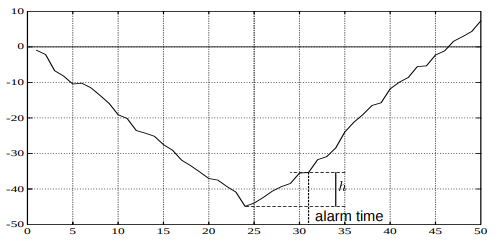
\includegraphics[width=\linewidth]{cusum-example}
		\caption{Example of a cumulative sum alarm from Basseville. \ref{basseville}}
		\label{fig:timeseries-waste}
		\end{figure}
	\end{column}
\end{columns} 
\end{frame}
